\documentclass[border=3pt]{standalone}
\usepackage{xcolor}
\usepackage{tikz}
\usetikzlibrary{arrows.meta,decorations.pathreplacing}

\definecolor{mathblue}{HTML}{1D4ED8}
\definecolor{mathred}{HTML}{DC2626}
\definecolor{mathgrid}{HTML}{CBD5E1}

\begin{document}
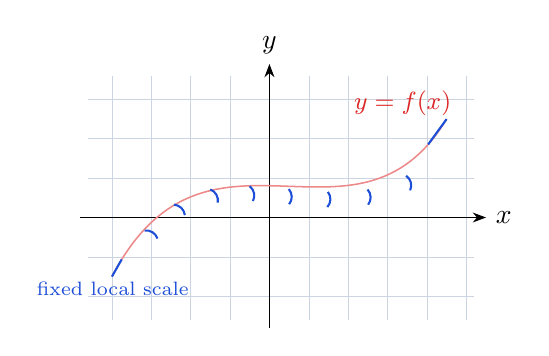
\begin{tikzpicture}[>=Stealth]
  \draw[mathgrid,very thin] (-2.3,-1.3) grid[step=.5cm] (2.6,1.8);
  \draw[-Stealth] (-2.4,0) -- (2.75,0) node[right] {$x$};
  \draw[-Stealth] (0,-1.4) -- (0,1.95) node[above] {$y$};

  \draw[mathred!55,line width=.55pt]
    (-2,-.75) .. controls (-.8,1.55) and (1.1,-.65) .. (2.25,1.25);
  \draw[mathblue,line width=.75pt,decorate,
    decoration={waves,segment length=5mm,radius=1.5mm,angle=40,
      pre length=2.5mm,post length=4mm,mirror,raise=1.5mm}]
    (-2,-.75) .. controls (-.8,1.55) and (1.1,-.65) .. (2.25,1.25);

  \node[mathred,anchor=west,font=\small] at (.95,1.45) {$y=f(x)$};
  \node[mathblue,anchor=east,font=\scriptsize] at (-.9,-.9)
    {fixed local scale};
\end{tikzpicture}
\end{document}
